
\chapter{Translation perception is modulated by eye movements that are partially scaled by fixation depth}
\chaptermark{}

\label{p4}

\newpage

\small {\bf Abstract}
It has been shown that the compensatory eye movements, that minimise retinal slip during self-motion, also serve as a cue for translation perception. However, to provide an adequate translation estimate, the brain must internally scale these ensuing eye movements by fixation distance. Using a 2AFC approach, we investigated whether the brain applies this scaling.  Participants ($n = 8$) were translated sideways in the absence of full-field optic flow but with gaze maintained on either a nearby or faraway target, that was either fixed in the world (world-fixed) or moved along with the body (body-fixed). Results show that translations were perceived shorter with gaze on nearby than faraway world-fixed targets, indicating that eye movements are not properly scaled in translation perception. Translation perception was not affected by the depth of body-fixed targets. Taken together, our results suggest that eye movements are merely a rudimentary cue to self-motion, with a compensation for fixation depth that is partial at best.

\vfill

\noindent\underline{ \hspace{4cm} }

\noindent This chapter is being prepared for publication \newline
\noindent {\bf Clemens, I.A.H.}, Selen, L.P.J., MacNeilage, P.R. and Medendorp, W.P. \citeyear{clemens2015b}. %Title. \emph{Journal}, volume(issue): from-to. \newline

\newpage


%%%%%%%%%%%%%%%%
% Introduction %
%%%%%%%%%%%%%%%%


\section{Introduction}

An accurate internal estimate of self-motion is required to navigate effectively through a complex three-dimensional environment. The vestibular system as well as optic flow provide essential information about self-motion \cite{gibson1955, benson1986, harris2000, israel1989, angelaki2005, carriot2013, chen2010}. During navigation, however, the eyes typically move to maintain visual acuity on important objects. These eye movements disturb the optic flow patterns. Using the oculomotor signal, the brain is able to account for these disturbances by internally separating optic flow into two components, one caused by self-motion and the other by eye movement \cite{warren1988, royden1992, freeman1998, lappe1999}.

When the eyes track world-centred objects, their angular displacement is directly related to the size of the motion of the observer \cite{schwarz1989, paige1998, mchenry2000, medendorp2002}. Because  the majority of fixations are on world-stationary  objects, we recently proposed that these tracking eye movements could also be used as a self-motion cue, in addition to optic flow and vestibular signals. To test this hypothesis, we compared self-motion perception in the absence of full-field optic flow during passively induced whole-body translations \cite{clemens2015a}. Our results showed that self-motion is underestimated during body-centred fixations (in which the eyes remain stationary in their orbits) compared to fixations on world-stationary objects (in which the eyes must move to maintain fixation).

Geometrically, eye movements that keep fixation on a world-centred target during lateral whole body translation (i.e. the linear vestibulo-ocular reflex; LVOR), must scale with fixation depth \cite{angelaki2004}. When fixating body-centred targets these eye movements must be suppressed irrespective of fixation distance \cite{angelaki2004}. Conversely, when fixating world-centred targets, the brain must internally scale the ensuing eye movement by fixation distance to serve as an adequate self-motion cue. Because we did not manipulate fixation distance in our previous study, we could not dissociate whether eye movements are used as a rudimentary cue for self-motion (i.e. without taking fixation depth into account), or are properly scaled in the mechanisms for self-motion perception.

In the present study, we investigate how fixation distance influences perception of self-motion during passive side-to-side translations. Using a psychophysical approach, participants had to indicate whether the second body displacement of two one-second translation intervals was smaller or longer than the first. We show that translation amplitude is perceived smaller when fixating a far compared to a nearby world-centred target, indicating that eye movements are not properly scaled in self-motion perception. Together with the observation that self-motion perception is not affected by the depth of a body-centred fixation target, we conclude that eye movements are merely a rudimentary cue to self-motion, with a compensation for fixation depth that is partial at best.


%%%%%%%%%%%
% Methods %
%%%%%%%%%%%


\section{Materials and methods}
\label{p4:sec:methods}

\subsection{Participants}

Eight naive participants (three male, five female), aged between 22 and 29 years, gave written informed consent to participate in the study. They were all free of any known vestibular or neurological disorder and had normal or corrected-to-normal visual acuity. Participants never received any feedback about their performance.  The experimental setup and methods used here are similar to those used in our previous paper on the influence of eye movement type on self-motion perception \cite{clemens2015a}. We only provide a brief summary here, and refer to our previous paper for further details.

\subsection{Experimental setup}

Participants were seated on a motorised linear sled with their body and head restrained such that the inter-aural axis aligned with the motion axis. The sled laterally translated participants following a minimum jerk profile of fixed duration (1 \si{\second}) and amplitudes ranging from 1 to 27 \si{\centi\metre}. Auditory cues were suppressed using white noise presented through in-ear head-phones. Experiments were conducted in complete darkness except for visual fixation points, projected by body- or world-fixed laser pointers on a black bar, either 50 or 200 \si{\centi\metre} in front of the participant and at eye level. Eye movements were recorded at 500Hz using an EyeLink II system (SR Research, Kanata, Canada). Eye position was calibrated before every session using 11 evenly spaced calibration points ranging from -22 to 22 degrees.


\subsection{Paradigm}

We used a two-alternative forced choice (2AFC) task to study the influence of fixation depth on the perception of linear translation. We tested two fixation depths: near (50 \si{\centi\metre}) and far (200 \si{\centi\metre}) and two different eye fixation conditions: world-, and body-fixed fixation. A trial contained two sequential motion intervals of equal duration (1 \si{\second}), with the motion in the same direction (either leftward or rightward).

%Fixation condition (world-, or body-fixed) was the same in both intervals, but a different fixation depth was presented in each. Participants had to judge whether the translation during the second motion interval was longer or shorter than in the first motion interval.

\begin{figure}
    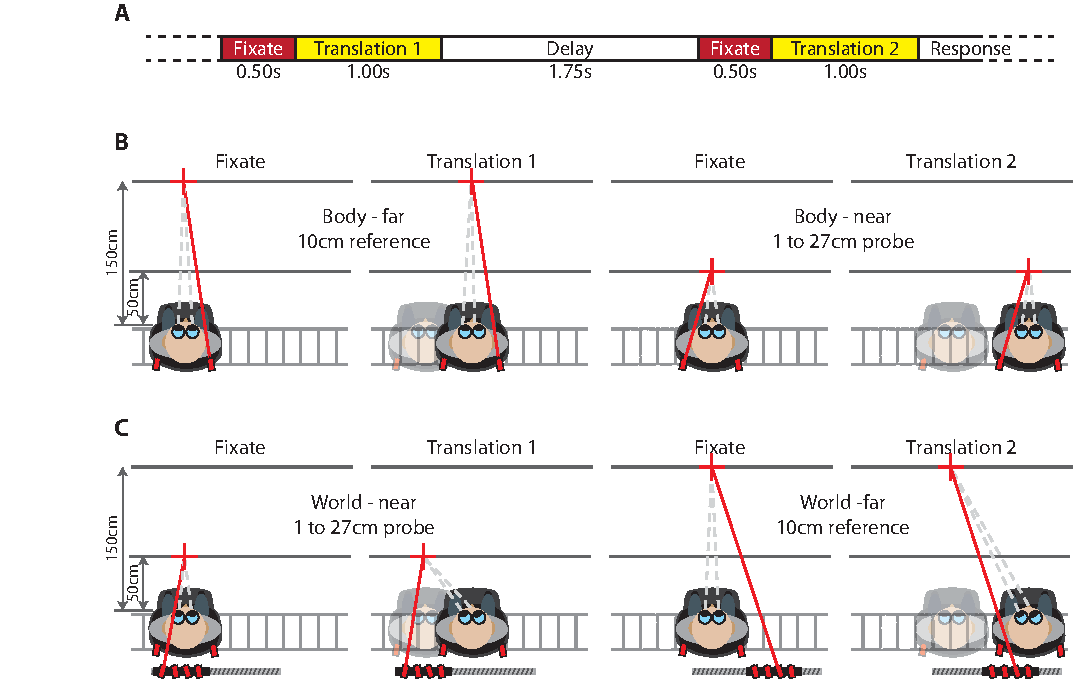
\includegraphics[width=1.0\textwidth]{src/paper4/p4_figure1.pdf}

    \caption{\panel{A} Time course  of key events within a single trial. In each of the two intervals, a 0.50 \si{\second} fixation period (red) precedes the lateral translation (yellow). A 1.75 \si{\second} long delay period (shown in white) separates the two intervals. After the second translation, the participant responded whether this second translation was longer or shorter than the first. \panel{B} and \panel{C} Top-view illustrating key events in a far versus near body-fixed fixation trial (\panel{B}) and a near versus far world-fixed fixation trial (\panel{C}). The first panel shows the initial fixation to the target (red cross) followed by a translation in the second panel. The third panel shows the initial fixation before the second movement interval followed by a translation in the fourth panel.}
    \label{p4:fig1}
\end{figure}

The timing of a single trial is shown in \panelref{p4:fig1}{A}. Every trial started with the onset of a central fixation point (i.e. aligned between the eyes), at a depth of 50 or 200\si{\centi\metre}, for 0.5 \si{\second}. Subsequently, the first 1\si{\second} motion interval commenced. During this translation, the fixation point either remained world stationary (world condition), or moved along with the participant (body condition).  Subsequently a 1.75 \si{\second} delay followed in which the sled was stationary and no  fixation light was shown. Next, a central fixation point reappeared at the other depth (50 or 200\si{\centi\metre}) than was used in the first interval. After 0.5 \si{\second}, the second 1 \si{\second} translation interval started, with the same fixation condition as in the first interval. After this second interval, the participant responded whether the second displacement was perceived longer or shorter than the first by moving a 1-dimensional joystick away from (longer) or towards (shorter) the body. Top-view illustrations of example body-centred and world-centred trials are shown in \panelref{p4:fig1}{B} and \hyperref[p4:fig1]{C} respectively.

\begin{table}
    \begin{tabular}{llll}
    Comparison & Reference & 1st interval & Direction \\
    \hline
    Body & Near & Reference & Right \\
    Near vs. far & & & Left \\
    & & Probe & Right \\
    & & & Left \\
    \cline{2-4}
	& Far & Reference & Right \\
    & & & Left \\
    & & Probe & Right \\
    & & & Left \\
    \hline
    World & Near & Reference & Right \\
    Near vs. far & & & Left \\
    & & Probe & Right \\
    & & & Left \\
    \cline{2-4}
	& Far & Reference & Right \\
    & & & Left \\
    & & Probe & Right \\
    & & & Left \\
    \end{tabular}

    \caption{List of the 2 main comparisons that we tested. The (10cm) reference movement was presented in either the first or the second interval. We also manipulated movement direction (leftward vs rightward) yielding a total of 16 trial types.}

    \label{p4:tab1}
\end{table}

% Should look at the 4 vs 16 in the next part, sounds confusing.
Across trials, we varied the order of the fixation depths and the order  of the reference and probe interval, resulting in four variations of both the world and body condition (see \tabref{p4:tab1}).

Leftward and rightward motion alternated between trials, but were not considered as variations of the condition. To determine the point of subjective quality (PSE), the size of the probe translation was adaptively chosen based on the participants' earlier responses (Psi method; \citeNP{kontsevich1999}). This was done separately for all 16 trial types (2 main conditions x 2 depth orders x 2 reference/probe orders x 2 movement directions; see Table 1). A total of 25 trials was collected per trial type yielding a total of 200 trials for each of the two main conditions.

These trials were presented in two one-hour sessions. To prevent dark adaptation, we turned on the lights for 5 \si{\second} after every 8 trials, and for at least 30 s after every 16 trials. Each of the 16 unique trial types were presented once in every block of 16 trials. After each block, the adaptive procedure determined which translation size to test in the following block. To increase the number of data-points available to the adaptive psychometric procedure at the beginning of the experiment, we collapsed across movement direction and reference order for the first 10 trials. After that, the procedure ran separately for the 16 distinct trial types.

\subsection{Data analysis}

For each combination of the two main conditions and the two reference/probe orders we computed the probability $P(x)$ of probe translation $x$ being  judged as longer than the reference translation. To summarise these data, we fit cumulative Gaussian functions to these probabilities, resulting in a total of four Gaussian functions per participant (see \tabref{p4:tab1}):

\begin{equation}
\label{p4:eq1}
P(x) = \lambda + (1 - 2\lambda) \frac{1}{\sigma \sqrt{2\pi}} \int_{-\infty}^{x}{e^{-(y-\mu)^2 / 2\sigma^2}}dy,
\end{equation}

The mean of the Gaussian, $\mu$, represents the point of subjective equality (PSE). The slope of the curve reflects the precision ($1/\sigma$) of reference-probe discrimination performance. Parameter $\lambda$, representing the lapse rate, accounts for stimulus-independent errors caused by subject lapses or mistakes and was restricted to small values ($\lambda < 0.06$). Fits were performed using the Psignifit toolbox \cite{wichmann2001,wichmann2001b}.

For each trial type (see \tabref{p4:tab1}), we also quantified the eye movements, corrected for drift based on initial fixation. We discarded trials containing blinks as well as trials in which final eye position exceeded two standard deviations from the condition's average. Based on these criteria, 12\% of all trials were discarded. Of the remaining trials, we computed the average ratio between the measured eye excursion, $\varphi_i$, and the angle that  the eyes would have  moved through had they perfectly tracked a world-stationary fixation target at the same fixation depth. The latter is computed by taking the arc-tangent of the actual translation distance, $m_i$, divided by the fixation depth, $d_i$, which for small $\varphi$ can be approximated by $g_c = \frac{\varphi_i m_i}{d_i}$. We computed this ratio, $g_c$, for every trial type $c$ (see \tabref{p4:tab1}). Ideally, for body-fixed trials, $g_c = 0$; and for world-fixed trials, $g_c = 1$.


\subsection{Model}

Using a straightforward model, we investigate to what extent fixation depth is taken into account in the contribution of eye movements to self-motion perception. As in \citeA{clemens2015a}, we model the perceived translation, $p_i$, as a weighted combination of a vestibular, $m_i$, and oculomotor estimate of translation, $\hat{\varphi}_i$ (\eqnref{p4:eq4}).

\begin{equation}
\label{p4:eq4}
p_i = \alpha_{d_i} \hat{\varphi}_i + (1 - \alpha_{d_i}) m_i
\end{equation}

Variable $i$ represents either the reference, $r$, or probe, $p$, interval. To serve as a veridical cue for self-motion, eye movements need to be scaled by the depth of fixation, $d$. This scaling is reflected by parameter, $\alpha_{d_i}$. If this parameter is the same across the two fixation depths, $d$, then there is no depth-dependent modulation of the oculomotor estimate of translation.

By definition, at the PSE, the probe translation is perceived as equal in length to the 10 cm reference translation, $p_r = p_p$. By substituting both sides by the right hand side of \eqnref{p4:eq4}, we obtain:

\begin{equation}
\label{p4:eq5}
\alpha_{d_r} \hat{\varphi}_r + (1 - \alpha_{d_r}) m_r = \alpha_{d_p} \hat{\varphi}_p + (1 - \alpha_{d_p}) m_p + \epsilon
\end{equation}

We fit \eqnref{p4:eq5} to the data using linear regression, finding one weight for each of the two fixation depths (that is, $\alpha_{50}$ and $\alpha_{200}$) that minimises the sum of squared errors ($\Sigma \epsilon^2$). Because these parameters can, in theory, contain both a depth-dependent and a depth-independent scaling, we compute their ratio, $\alpha_{200}/\alpha_{50}$, to remove any depth independent components. In case of perfect compensation, the expected ratio is $200/50 = 4$, while in case of depth-independent scaling it is 1.


%%%%%%%%%%%
% Results %
%%%%%%%%%%%


\section{Results}

In a recent study we have shown that eye movement signals contribute to the perception of body translation, even in the absence of optic flow or a visual fixation point \cite{clemens2015a}. Because eye rotations must be scaled by target depth ($\varphi d = T$) to serve as an adequate translation cue, we tested self-motion perception for near (50 \si{\centi\metre}) and far (200 \si{\centi\metre}) fixations. Participants were presented with two subsequent translations \figref{p4:fig1} while they kept fixation on a world- or body-stationary target that was presented either nearby or far away. After the two translation intervals, participants had to judge whether the second translation was longer or shorter than the first.

\begin{figure}
    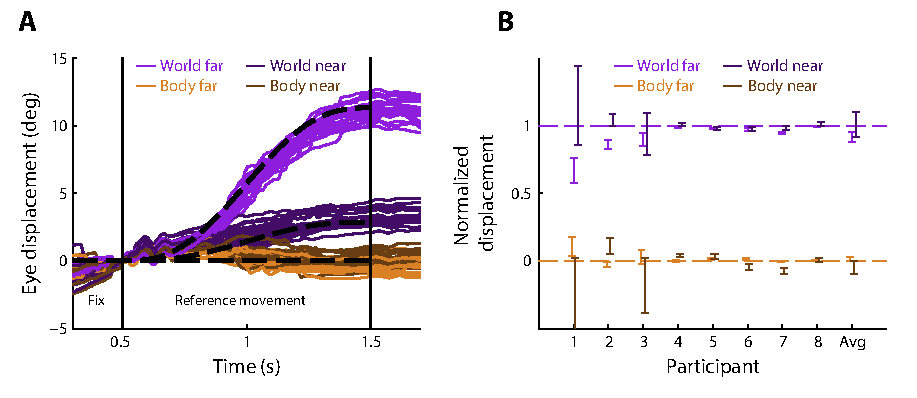
\includegraphics[width=1.0\textwidth]{src/paper4/p4_figure2.pdf}

    \caption{\panel{A} Actual (solid lines) and ideal (dashed lines) eye movement traces of one participant in the body-fixed (brown and orange) and world-fixed conditions (purple and pink). Gaze was directed at a near (brown and purple) or far (orange and pink) target. All traces shown are for 10 \si{\centi\metre} reference displacements. \panel{B} Normalised eye position for each participant (\textpm 95\% confidence interval) at the end of the translation interval for the near and far world fixed targets (purple and pink respectively) as well as the near and far body fixed fixation targets (brown and orange respectively). In addition, the average \textpm SE across all participants is shown. Zero indicates the eyes remained stationary relative to the body, and one indicates the eyes followed the near world fixed target perfectly.}
    \label{p4:fig2}
\end{figure}

We first investigated the ability of participants to fixate body and world stationary targets. \panelref{p4:fig2}{A} depicts exemplar eye traces for the 10cm reference translation with nearby and far fixation points in both the body and world condition. Changes in gaze are largely absent in the body near and body far conditions (brown and orange traces respectively), as required. During the world conditions, the eye excursions were large when fixating nearby targets and small when fixating far away ones (purple and pink traces respectively), which reflects the geometrical constraints.

We normalised the eye movement data by taking the average ratio between the measured eye excursion and the geometrically required eye displacement were the target world stationary. \panelref{p4:fig2}{B} shows that these normalised eye displacements are about zero during body fixed fixations (brown and orange) and close to one in the world fixed fixations (purple and pink data points), for all participants. The question is whether these eye movements are inversely scaled by fixation depth in order to interpret them as linear self-motion cues.

\begin{figure}
    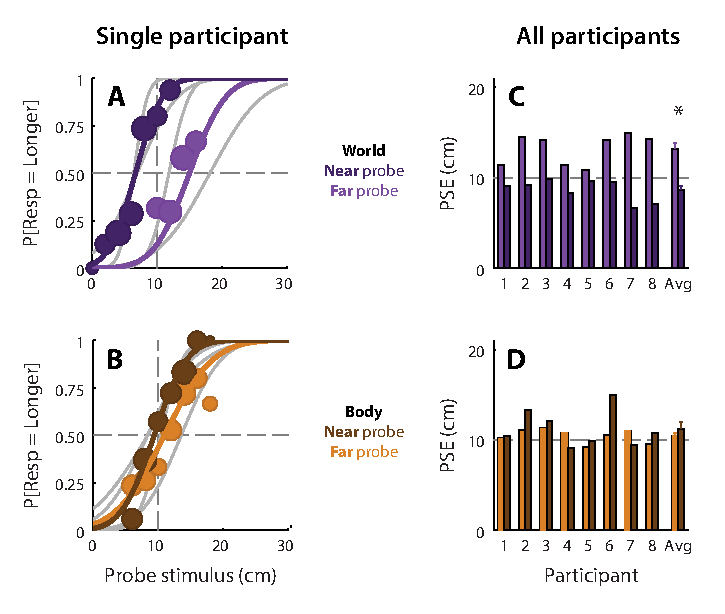
\includegraphics[width=1.0\textwidth]{src/paper4/p4_figure3.pdf}

	\caption{\panel{A} and \panel{B} Psychometric curves (coloured lines) and associated binned data (circles) for one participant. Circle size represents the amount of trials within the bin. Psychometric curves before collapsing across reference order are shown as gray lines. \panel{A} World-fixed condition (purple) while fixation was either near (dark) or far (light). \panel{B} Body-fixed condition (brown) while fixation was either near (dark) or far (light).
	\panel{C} and \panel{D} Individual and average points of subjective equality (PSEs). Colour scheme matches panels A and B.
	}
	\label{p4:fig3}
\end{figure}

\figref{p4:fig3} illustrates psychophysical data on self-motion perception of a single participant for the two-fixation depths in both the world (\panelref{p4:fig3}{A}) and body condition (\panelref{p4:fig3}{B}). Lighter and darker colours indicate which fixation depth was the reference translation (see figure legend). The influence of fixation depth is characterised by a shift of the psychometric functions relative to the 10 \si{\centi\metre} reference translation (i.e. the PSE). For example, the rightward shift of the pink curve in \panelref{p4:fig3}{A}, representing the world-condition, means that with a far target a longer translation (\about15 \si{\centi\metre}) was required to be perceived equivalent to a 10 \si{\centi\metre} reference translation with nearby fixation. Likewise, the leftward shift of the purple curve indicates that a shorter translation with near fixation (\about6 \si{\centi\metre}) is required to be perceived the same as the 10 \si{\centi\metre} reference translation with far fixation. Together, these opposite biases suggest that translations are perceived shorter for fixations further away. For the body condition, no shift of the psychometric curves is visible (\panelref{p4:fig3}{B}), indicating that fixation depth (i.e. near versus far) has no effect in absence of eye movements.

Similar results were obtained for all participants, as shown by the individual PSEs (right column of \figref{p4:fig3}). Statistical significance of the effects of fixation depth was evaluated by comparing PSEs for the two fixation depths using a paired t-test. PSEs  differed significantly between the two fixation depths in the world condition, $t(7) = 5.42$, $p < 0.01$ (\panelref{p4:fig3}{C}), but not in the body condition, $t(7) = -1.17$, $p = 0.28$ (\panelref{p4:fig3}{D}), confirming the single subject results (\panelref{p4:fig3}{A and B}). Thus, increasing fixation depth does not influence self-motion perception during body-stationary fixations, but causes self-motion to be perceived as shorter during world-stationary fixations.

\begin{table}
    \begin{tabular}{l|lll|l}
	Participant & $\alpha_{50}$ & $\alpha_{200}$ & $\frac{d_{200}}{d_{50}}$ & $\alpha$ \\
    \hline
	1 & 0.37 & 0.25 & 1.46 & 0.27 \\
	2 & 0.51 & 0.41 & 1.25 & 0.27 \\
	3 & 0.36 & 0.30 & 1.22 & 0.35 \\
	4 & 0.14 & 0.29 & 0.49 & 0.06 \\
	5 & 0.11 & 0.04 & 2.79 & 0.13 \\
	6 & 0.49 & 0.15 & 3.34 & 0.33\\
	7 & 0.40 & 0.53 & 0.76 & 0.58 \\
	8 & 0.42 & 0.35 & 1.25 & 0.21 \\
    \end{tabular}

    \caption{Best-fit parameter values for 50 and 200 \si{\centi\metre} fixation distances, $\alpha_{50}$ and $\alpha_{200}$ respectively (see \eqnref{p4:eq5}), and their ratio, $\alpha_{200} / \alpha_{50} = d_{200} / d_{50}$, for each participant. Best-fit parameter values, $\alpha$, from our previous paper \protect\cite{clemens2015a} are included for reference.}

    \label{p4:tab2}
\end{table}

\begin{figure}
    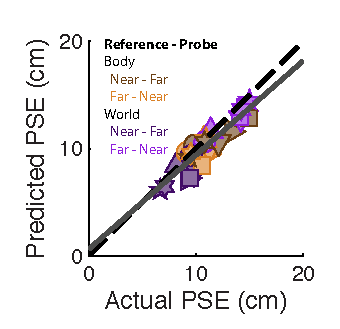
\includegraphics[width=0.5\textwidth]{src/paper4/p4_figure4.pdf}

	\caption{Eye movement based prediction for the PSE plotted against the actual PSE. A data point (symbol) is shown for each participant (symbol shape) and condition (symbol colour) pair, following the same colour scheme as in \figref{p4:fig3}. The identity line, corresponding to a perfect prediction is shown (solid line) as well as the best fit line (dashed).}
	\label{p4:fig4}
\end{figure}

We used a simple linear model to quantify to what extent eye movements are scaled by fixation depth in order to serve as a linear self-motion cue (see \nameref{p4:sec:methods}). This model describes the perceived translation distance as a weighted average of a vestibular estimate, equal to the actual translation, and an oculomotor-based estimate. The latter estimate depends on the eye excursion which should be scaled by fixation depth to serve as a valid cue. Our model contained two weighting parameters, $\alpha_{50}$ and $\alpha_{200}$, one per fixation depth (see \tabref{p4:tab2} for best-fit values). Using these parameters we predicted the PSEs, i.e. $m_p$ in \eqnref{p4:eq5}, and plotted them against the actually observed PSEs in \figref{p4:fig4}. The positive correlation ($\rho = 0.92$, $p < 0.01$) between observed and predicted PSEs shows that our simple model does reasonably well in predicting perceptual performance.

\begin{figure}
    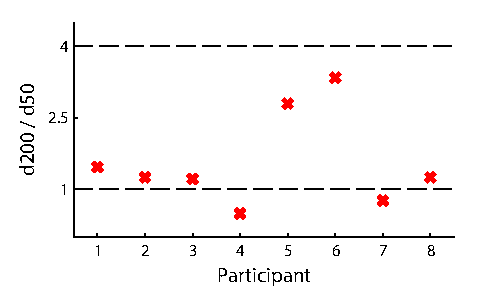
\includegraphics[width=0.5\textwidth]{src/paper4/p4_figure5.pdf}

	\caption{Ratio between near and far parameter values, $\alpha_{200} / \alpha_{50} = d_{200} / d_{50}$ for every participant. Both perfect depth compensation, $\alpha_{200} / \alpha_{50} = 200 / 50 = 4$, as well as the lack thereof, $\alpha_{200} / \alpha{50} = 1$, are represented by a dashed line.}
	\label{p4:fig5}
\end{figure}

By examining the ratio of these weighting parameters, we remove any depth-independent contributions. In absence of  depth scaling, i.e. when $d_{50} = d_{200}$, the ratio should be one. For perfect compensation, that is when $d_{50} = 50  \wedge d_{200} = 200$, the ratio should be $4$. The actual ratio between $d_{50}$ and $d_{200}$ is plotted for each participant in \figref{p4:fig5}. While two participants show moderate compensation for depth, the majority of participants show no clear sign of scaling of eye movements by fixation distance. This is consistent with the observation that translations are perceived shorter with far compared to near fixations in the world condition.


%%%%%%%%%%%%%%
% Discussion %
%%%%%%%%%%%%%%


\section{Discussion}

% Relation to previous work / Should rewrite this paragraph!
In our previous study, we demonstrated that oculomotor signals play a substantial role in the perception of translation, even in the absence of optic flow or any other visual stimulation \cite{clemens2015a}. Although the vestibular system provided the most significant contribution, oculomotor signals were shown to account for about 20\% of the overall percept. Because these experiments were performed with a single fixation depth, it was not clear whether the brain weighted the oculomotor signal in a depth-dependent manner when using it as a translation cue, or merely uses the signal as a rudimentary cue to self-motion. In the present study we tested between these two possibilities.

% Basic observations
We assessed translation perception during both body- and world-fixed fixation at two different fixation depths. Our results show that self-motion was underestimated when comparing far and near fixation trials in the world-fixed condition, which argues against a proper scaling of the eye movement signal. Fixation depth did not influence translation perception during body-fixed fixation (where eye movements are virtually absent).

% Model results
To quantify the relative depth-dependent scaling of eye movements for nearby and far away fixation targets, we fitted a straightforward linear model to the perceptual responses based on the oculomotor behaviour across four conditions. While two participants show partial scaling, the other six participants did not show any sign of scaling. Thus, we conclude that while oculomotor signals provide a robust cue to translation perception, they are not properly scaled by fixation depth.


\subsection{Relation to other studies}

% Relation to Clemens, 2015
\begin{figure}
    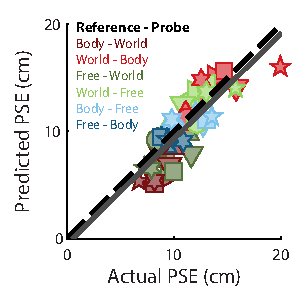
\includegraphics[width=0.5\textwidth]{src/paper4/p4_figure6.pdf}

    \caption{Predicted versus actual PSEs for Clemens \protect\citeyear{clemens2015a} using parameter $\alpha_{50}$ from the present paper. A data point (symbol) is shown for each participant (symbol shape) and condition (symbol colour) pair, following the same colour scheme as in \protect\figref{p3:fig2}: Body-world comparison; body reference, dark red; world reference, light red. World-free comparison; world reference, light green; free reference, dark green. Body-free comparison; body reference, dark blue; free reference, light blue.}
    \label{p4:fig6}
\end{figure}

In our previous experiment we compared translation perception with body-fixed versus world-fixed fixations at near depth (50 \si{\centi\metre}) only \cite{clemens2015a}. \figref{p4:fig6} shows how well our $\alpha_{50}$ parameter explains the data in our previous paper. The positive correlation between the actual PSEs in the previous study and those predicted using the model of the present paper ($\rho = 0.60$, $p = 0.06$) adds confidence to the parameter values presented here. The average difference between the values found here and those reported previously (see \tabref{p4:tab2}) is 12 \textpm 8 percent-points, which is relatively small given the independent measurements.

% Relation to the VOR
The function of the LVOR is to keep the eyes stable in the world during linear translation \cite{paige1989,busettini1994,paige1998}. Because it also needs to scale with fixation depth \cite{angelaki2004}, it is possible that the LVOR and self-motion perception have the same underlying signal. Because of the visual fixation point in our paradigm, visual following mechanisms may even augment the LVOR compensation. If the oculomotor signal generated by the LVOR is used for self-motion perception, one would expect that the LVOR compensation at 50 and 200cm closely relate to the corresponding oculomotor weights in the present study (see \figref{p4:fig5} and \tabref{p4:tab2}). To further explore this, we derived the LVOR gains for 50 and 200 \si{\centi\metre} from Paige et al. \citeyear{paige1989} and computed their expected depth ratio, $d_{200} / d_{50}$. This ratio, 1.87, is in between the ratio of the 6 participants who did not show any sign of scaling ($\frac{d_{200}}{d_{50}} = 1.07 \pm 0.16$) and the 2 participants that did show scaling ($\frac{d_{200}}{d_{50}} = 3.06 \pm 0.27$), suggesting that our effect might share a pathway with the LVOR.


\subsection{Alternative explanations}

It is important to point out that while the vestibular signal and thus noise is constant for a given translation distance, the noise in the associated oculomotor estimate might change with fixation distance because the magnitude of the eye movement is modulated by fixation depth and may show signal-dependent noise.

If this were the case, the nearby world-fixed fixations would cause larger eye movements with more noise compared to the far world-fixed fixations with smaller eye movements. The oculomotor based translation estimate would be weighted less for near versus far fixation, potentially explaining the partial compensation for fixation depth we have observed. In addition, the noise levels in the oculomotor estimate could also depend on fixation depth itself: the retinal displacement of a world stationary fixation point decreases with fixation depth, making it less informative about the amount of self-motion. The noise level in the oculomotor estimate would therefore be higher for far away compared to nearby fixation points. For world stationary targets, this would predict an underestimation of self-motion while fixating far away compared to nearby, which is in line with our observations. However, it also predicts a similar effect for body stationary targets. As no such effects between the near and far body stationary fixation targets have been observed, we consider it an unlikely alternative explanation.

Could the lack of scaling be explained by how participants perceive the distance of the fixation points? Because the difference between body- and world-fixed fixation points is reduced at far fixation distances, the lack of scaling could - in theory - be explained by participants incorrectly perceiving both the body- and world-fixed far fixation points as being body-fixed. We consider this an unlikely explanation, because the target displacement associated with a world-fixed target was between 0.3 and 8.5 degrees in our experiment, which is easily perceived. This adds confidence to our claim that eye movements influence self-motion perception, but with moderate to no scaling for fixation depth.
